% kompiliert mit XeLaTeX
\documentclass[
12pt, % font size
parskip=half, % space between paragraphs instead of indentation
digital, % digital or print
oneside, % oneside / twoside
%	openright, % openright for title page and subsequent chapters on right pages in twosided layout
]{bsc}

\usepackage {xltxtra}
\usepackage{microtype}
% Package für Bilder
\usepackage{graphicx}
\usepackage{enumitem}

\title{Understanding}
\author{Max SImon}
\date{August 21, 2017}

% Mathe
\usepackage{amsmath, amssymb, booktabs, hyperref, subcaption, siunitx}

\bibliography{../Paper}

% Code
\usepackage{listings}

\newcommand{\diff}{\text{d}}
\newcommand{\pip}{PI(4,5)P$_2$}
\newcommand{\acid}[2]{#1$^{#2}$}
\newcommand{\gromacs}{GROMACS}
\newcommand{\pope}{POPE}
\newcommand{\popc}{POPC}
\newcommand{\forceunit}{\si{\kilo\joule/\mole/\nano\metre}}

%\newcommand{\fourier}[1]{\mathcal{F}\left( #1 \right)}
%\newcommand{\revfourier}[1]{\mathcal{F}^{-1}\left( #1 \right)}


\captionsetup[subfigure]{labelformat=simple, labelsep=colon}
\renewcommand{\thesubfigure}{Figure~\thefigure \alph{subfigure}}

\includeonly{introduction/characterisation}

\begin{document}
	
\chapter{Introduction}
\section{Focal adhesion kinase}
Focal adhesions (FA) are macromolecular protein complexes which act as a connection hub between the cell, i.e. the cytoskeleton, and the extracellular matrix (ECM). They enable the cell to performing tension forces, but can also trigger mechanical stimuli from the ECM. One important protein associated to FA is the focal adhesion kinase (FAK). Due to its importance in e.g. cell migration and development \autocite{pap004}, it is of large interest for science.\\% smth about cancer and invasive tumors? \autocite{cancerFAK}.
\\
FAK consists of four major domains (see \autoref{TOBEADDED}): a FERM domain, a tyrosine kinase domain, a proline rich region and a focal adhesion targeting (FAT) domain.\\
FERM (4.1 protein, ezrin, radixin and moesin) is a common protein domain, which targets proteins to membranes \autocite{fermdomain} and consists of three subdomains F1, F2 and F3. In the F2 subdomain there is the basic patch  ($^{216}$KAKTLRK$^{222}$), which is a prominent binding site for phosphatidylinositol-4,5-bisphosphate (\pip), a phospholipid generated locally in FA \autocite{pap001}.\\
The kinase domain consists of the C-lobe, the activation loop and the N-lobe. The activation loop contains \acid{Y}{576}\,and \acid{Y}{577}, which have to be phosphorylated for a maximal activity of the kinase \autocite{tyrosinePhosphor}.\\
FAT is linked to the kinase by the proline rich region. FAT targets to FA by interacting with talin an paxillin, which are proteins associated with FA \autocite{fatdomain}.\\
\\
For an activation of FAK \acid{Y}{576,577} have to be phosphorylated. This is suppressed by the FERM domain, which shields the active loop. Therefore activation of FAK requires an conformational change in the interface of FERM and kinase domain. % describe allosteric, mechanosensing?
\section{Previous work}
\chapter{Methods}
Because the measurable time- and length scale of biological experiments are usually larger than those of the system, the dynamics in the system can only be measured indirectly. To get a more precise insight into the specific processes, Molecular dynamics simulation (MD) are a suitable tool.\\
In the following section the main concepts of MD and characteristics of the used models are outlined, with a special focus on the \martini{} force field. Nevertheless, this can only be a small survey in the scope of this thesis. Because \gromacs{} (\textit{GROningen MAchine for Chemical Simulations}) \autocites{gromacs1, gromacsManual} was used as MD engine in this thesis, the following explanations refer to \gromacs{} conventions and features. 
\subsection{The physics of MD}
In MD atoms are modelled as solid beads, which comprise the nucleus as well as the electron shell and follow classical equations of motion. Due to this implicit treatments of electrons, Quantum mechanical (QM) effects, such as excitation or electron transfer processes, are not accessible in MD. However, the beads are parametrized by effective parameters motivated by QM or experiments \autocite[p. 127f]{greenBook}.\\
Newtons equation of motion can be turned into two first order differential equation
\begin{align}
	\label{eq:eq_of_mot_first_order}
	\frac{\diff \vec{r}_i}{\diff t} = \vec{v}_i \\
	m_i \frac{\diff \vec{v}_i}{\diff t} = \vec{F}_i
\end{align}
which can be integrated numerically with e.g. Leapfrog- or Verlet integration scheme. Both are time reversible and symplectic, which ensures a small long term error in energy conservation \autocite[p. 72ff]{UnderstandingMD}. The force acting on particle $i$ is given by the potential $V$ at its position. In MD bonded and non-bonded interactions contribute to this potential, but also external forces can be applied.
\begin{align}
	\vec{F}_i = - \frac{\partial V}{\partial \vec{r}_i} = - \frac{\partial}{\partial \vec{r}_i} \left(V_\text{bonded} + V_\text{non-bonded} + V_\text{external}\right)
\end{align}
\subsubsection{Bonded interactions}
Bonded interactions act intramolecularly and describe chemical bonds. They can occur between two, three or four particles and refer to bond stretching, bending and torsion respectively. An illustration can be found in \autoref{md:fig_bonds}.\\
\\
Deviations of the bond length $r$ from an equilibrium distance $r_0$ results in potential energy, which is usually described by a harmonic oscillator with the force constant $k_\text{dist}$.
\begin{align}
V_{\text{dist, bond }i} = \frac{k_{\text{dist}}}{2}\left( r - r_{0} \right)^2
\end{align}
For larger deviations a Morse potential, which assumes an exponential decay of the potential energy, is more precise, but has a much higher computational cost.\\
\\
Bending of a chemical bond refers to deviations of the angle between three bonded $\theta$ partners from an equilibrium angle $\theta_0$. The resulting harmonic potential is usually described by a harmonic oscillator as well.
\begin{equation}
V_\text{angle} = \frac{k_\text{angle}}{2}\left( \theta - \theta_0 \right)^2
\end{equation}
The dihedral angle describes the angle between two planes, which go through 3 beads respectively and have 2 beads in common. Therefore it can be understood as a torsion angle, but can also be used to preserve plane rings and the chirality of four particle groups. The resulting potential energy is usually approximated with a periodic approach
\begin{equation}
V_{\text{dihedral, periodic}} = \frac{k_\text{dihedral}}{2}\left(1 + \cos\left(n \phi - \phi_0 \right)\right)
\end{equation}
where $k_\text{dihedral}$ describes the energy barrier for turning the dihedral angle, $n$ the number of minima in the energy function (multiplicity) and $\phi_0$ a phase factor \autocite[p. 71-83]{gromacsManual}.
%
%
%
\begin{figure}
	\subcaptionbox{\label{md:fig_bonds}}[0.5\textwidth]{
		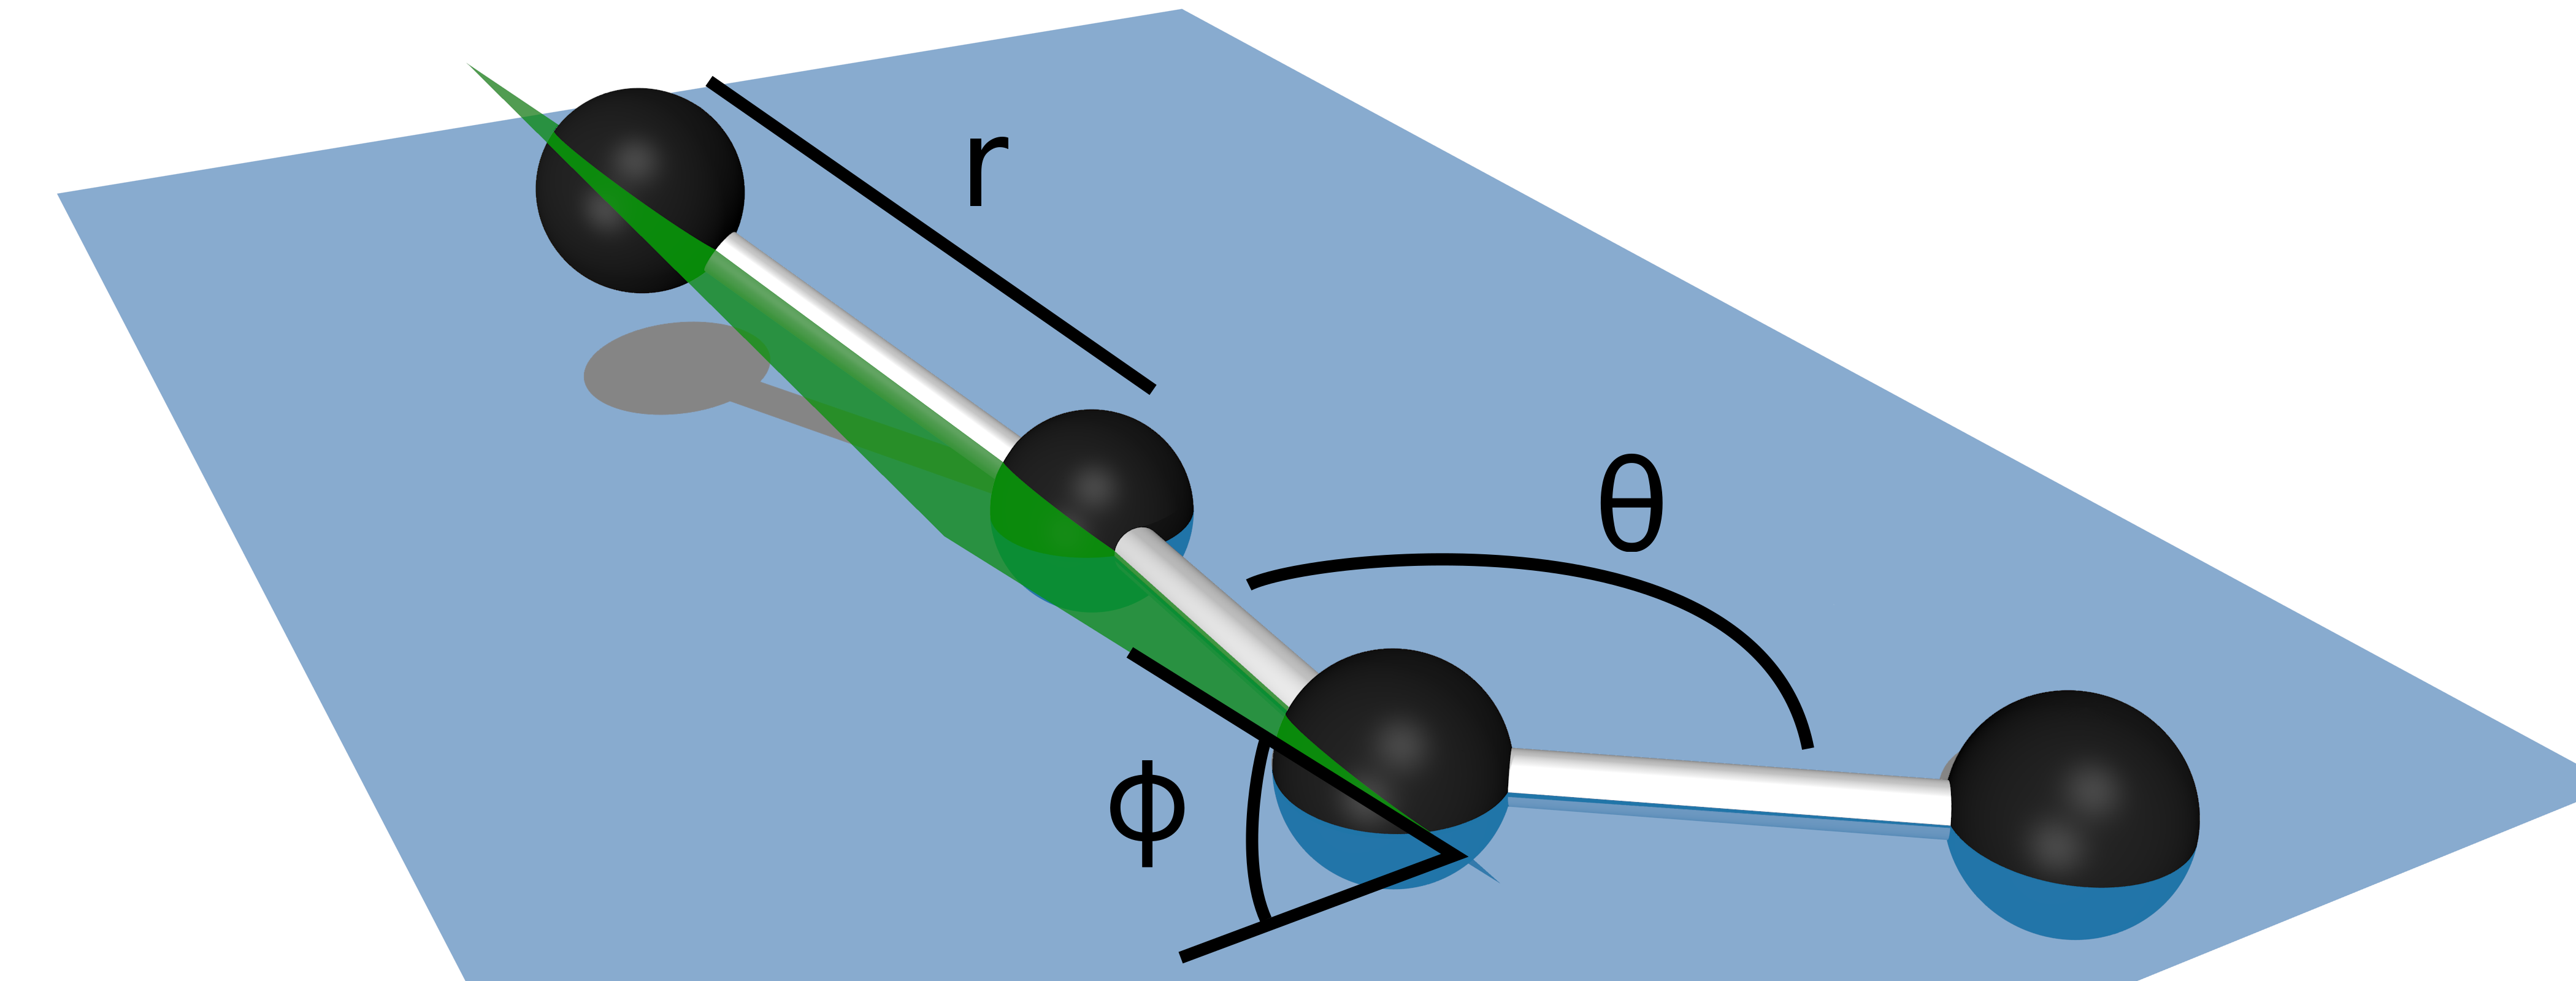
\includegraphics[height=3cm]{figures/introduction/fig_bonds}
	}\hfill%
	\subcaptionbox{\label{md:fig_pot}}[6cm]{
		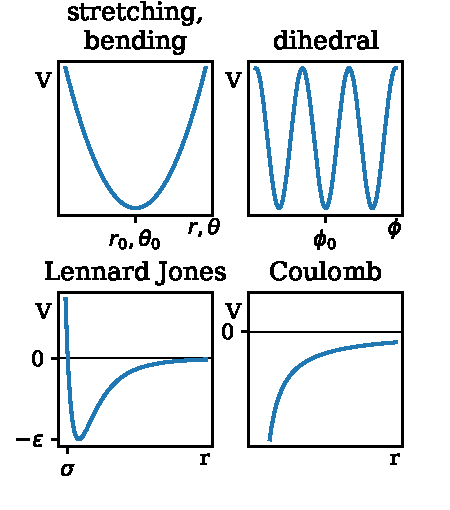
\includegraphics[height=6cm]{figures/introduction/fig_potentials}
	}%
	\nicecaption{Interactions in MD}{(\subref{md:fig_bonds}): Illustration of stretching $r$, bending $\theta$ and the dihedral angle between blue and green plane $\Phi$. (\subref{md:fig_pot}): schematic course of contributing potentials}
	\label{md:figs}
\end{figure}
%
%
%
\subsubsection{Non-bonded interactions}
Non-bonded interactions are present between all atoms in the system and act pairwise. In MD Pauli repulsion, van der Waals (vdW) forces and electrostatic forces are taken into account.
The Lennard-Jones potential combines Pauli repulsion ($r^{-12}$ term) and the vdW force ($r^{-6}$ term).
\begin{equation}
V_\text{Lennard-Jones} = \sum_{\text{non-bonded pairs i,j}} 4 \epsilon\left(\left(\frac{\sigma}{r_{ij}}\right)^{12} - \left(\frac{\sigma}{r_{ij}}\right)^6\right)
\end{equation}
$\epsilon$ is related to the potential depth and $\sigma$ to the potential range (\autoref{md:fig_pot}).\\
\\
The Coulomb potential is given by
\begin{equation}
V_\text{Coulomb} = \frac{q_1 q_2}{4 \pi \epsilon_0 \epsilon_r r}
\end{equation}
where $q_1$, $q_2$ are the (partial) charges of the interacting particles, $r$ their distance and $\epsilon_r$ the relative dielectric constant \autocite[p. 65-71]{gromacsManual}.\\
\\
In general non-bonded interactions act between all atoms in the system, which imply a very large computational cost.\\
The easiest solution for this problem is to use a cut-off radius $r_c$. Particles beyond this radius are not taken into account. This can be implemented very efficiently with a Verlet neighbour lists. For each particle a neighbour list is created, which contains all particles inside a second radius $r_v$ with $r_v > r_c$. This reduces the number of distance calculations a lot. The lists are updated, if the maximal displacement in the system is larger than $r_v - r_c$.  The application of a cut-off radius is suitable especially for Lennard-Jones potential as it decays very rapidly and $r_c$ can be chosen very small \autocite[p. 144]{greenBook}.\\
Because the electrostatic potential is proportional to $1/r$ the use of a cut-off radius would lead to large jumps in the potential. That is why long range interactions have to be considered, which can be effectively done with Particle Mesh Ewald (PME) summation \autocite{pme}. Particle mesh methods in general split the electrostatic potential up into a short range and a long range part via a switching function. The short range part can be calculated with a small cut-off radius in real space. The long range part however is calculated by solving the Poisson equation of the actual charge distribution, for which a discrete grid (mesh) is used. In contrast to other particle mesh methods, this grid is transformed to Fourier space in PME with FFT techniques. Here the solution of the Poisson equation is a sum over the gridpoints. Afterwards the potential can be back transformed into real space. The use of PME requires of course periodic boundary conditions, which are described in \autoref{subsec:pbc} \autocite[p. 246-251]{greenBook}.
\subsubsection{External forces}
With \gromacs{} it is possible to perform pulling forces onto groups of atoms in the system. In this thesis pulling was used to bias distances between groups. For this \gromacs{} provides an option to apply an umbrella potential to two groups which yields in a force proportional to the deviation of the distance between the groups from a reference distance. The force can be applied on one or two spatial dimensions only or along a predefined vector and the reference distance can change in time  \autocite[p. 154-159]{gromacsManual}.
\subsection{Force fields}
The parameters for the potentials described above are provided by force fields. There is a wide range of force fields, which are optimized for different application fields. In this thesis tow different ones, \charmm{} and \martini{}, are introduced.\\
\\
Force fields define specific atom types, which allow a mapping of atoms (particles in physical system) onto beads (particles used in the simulation). This mapping can take the environment of the particle (binding partners, solvents, nearby charges a.o.) into account, but can also neglect details by f.e. mapping several atoms to one bead (coarse-graining).\\
Force fields can be distinguished in non-polarizable and polarizable force fields. Latter offer the possibility to model electronic polarization, f.e. with additional shell beads. Orientational and geometric polarisation are also accessible with non-polarizable force fields since they only rely on partial charges \autocite[p. 215ff]{greenBook}.\\  
Force fields do not only define the atom types and their properties, but also all parameters for the calculation of the potential, namely force constants, equilibrium distances a.o. Therefore force fields define the physics of the system.
\subsubsection{All-atom and the \charmm{} force field}
\charmm{} \autocites{charmm36_protein}{charmm36_lipids} (C36) is part of the CHARMM (\textit{Chemistry at HARvard Macromolecular Mechanics}) MD engine and was published in 2010. In C36 all atoms are considered (all-atom force field). Parameters were mainly optimized to structural experimental data, such as nuclear magnetic resonance (NMR) or X-ray data, but also QM and semi empirical QM calculations were used (e.g. for dihedral angles of the sidechains of proteins \autocite{charmm36_protein} and partial charges of lipids \autocite{charmm36_lipids}).\\
All simulations for optimizing have been done with a time step of 2$\si{\femto\second}$. Therefore very detailed dynamics are still included in the simulations.\\
\\
For all simulations the TIP3P water model \autocite{tip3p} was used, which was also used in the parametrisation of C36. Here each water molecule is modelled with three partially charged beads.
\subsubsection{Coarse graining and the \martini{} force field}
\label{subsub:coarsegraining}
The \martini{} force field \autocites{martini}{martini22}{martini22_lipids} is one of the most famous coarse graining force fields. It maps usually four heavy atoms onto a single bead (\autoref{md:martinimapping}), which implicates of course a loss of chemical information, but also an enormous reduction of computational cost. With this approach much larger time- and spatial scales are accessible for MD simulations.\\
%
%
%
\begin{figure}
	\centering
	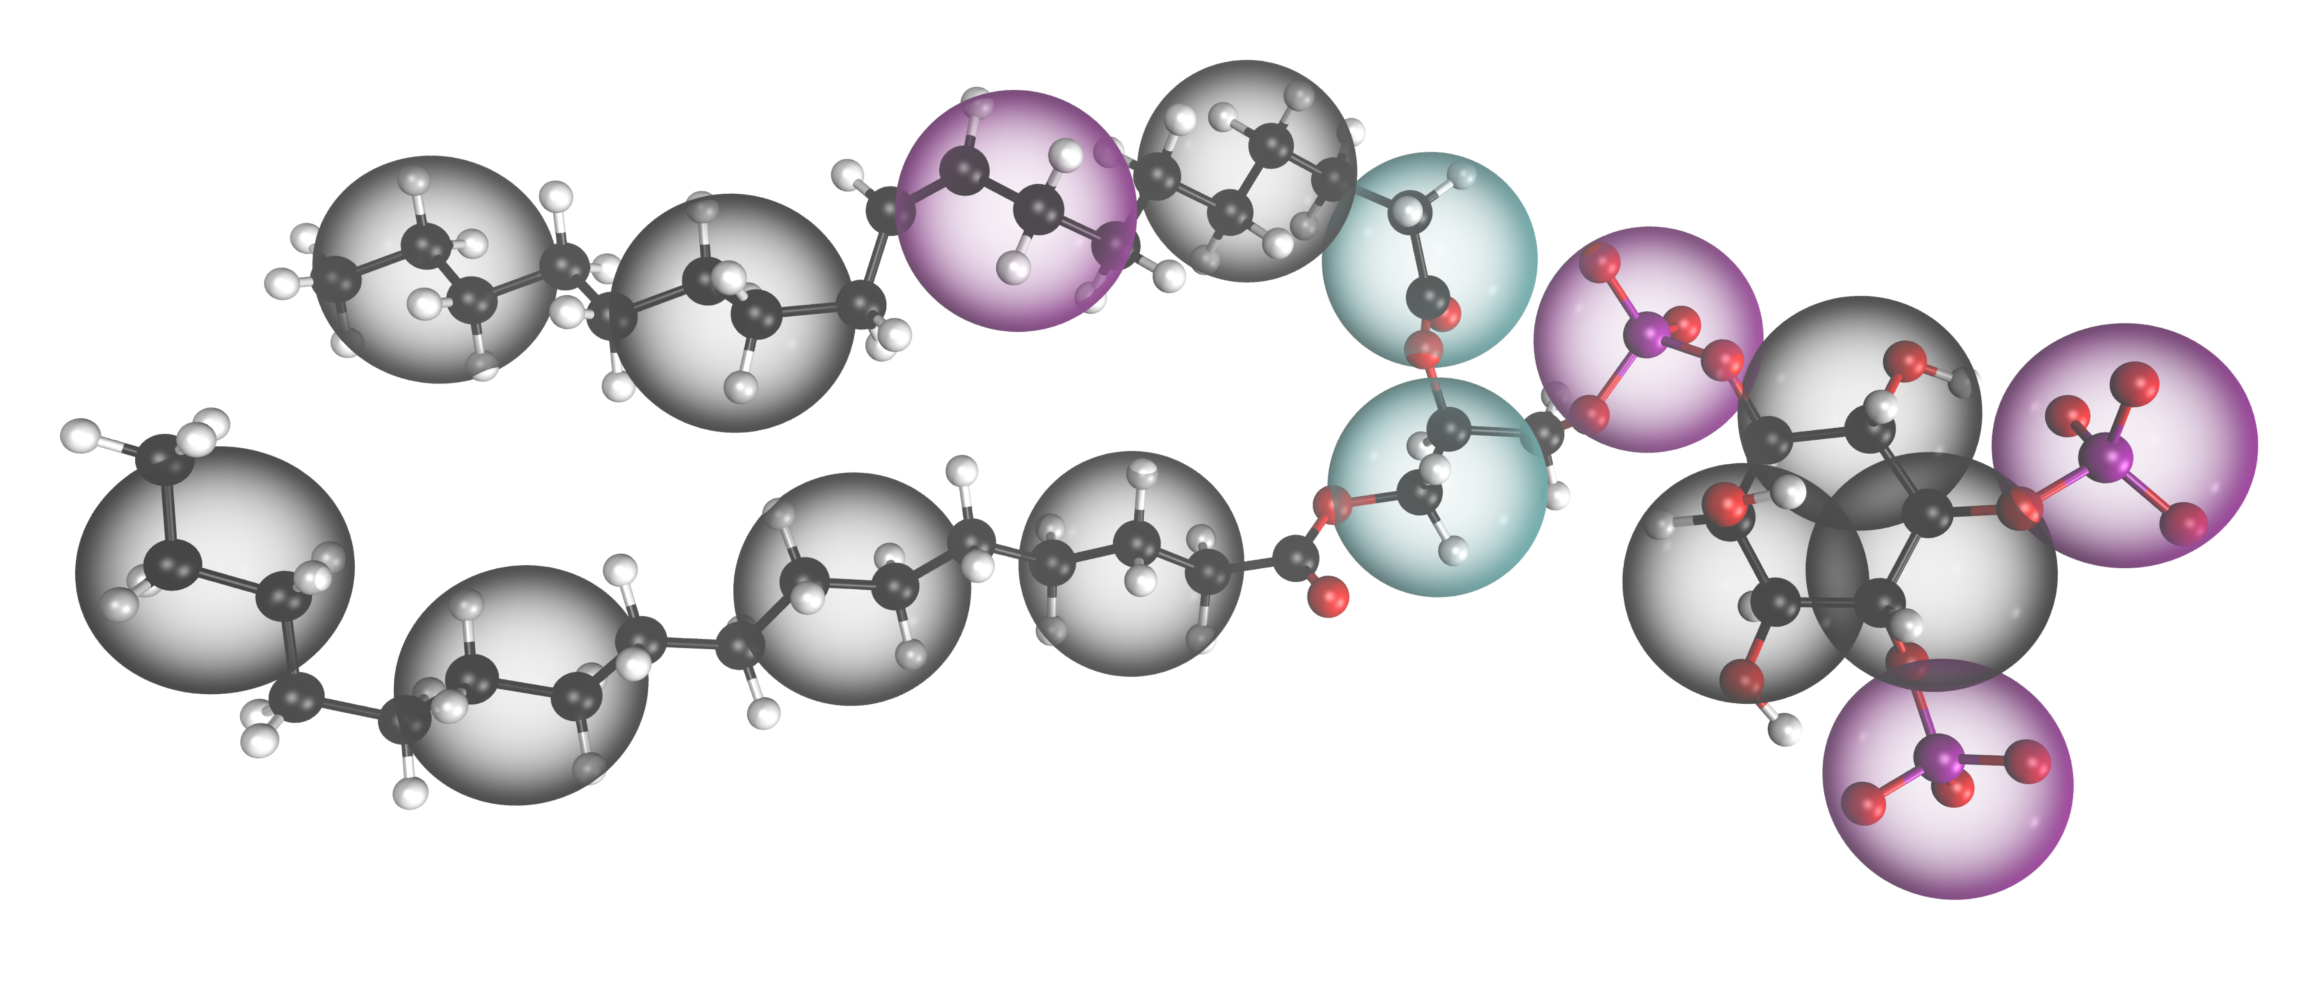
\includegraphics[width=.5\textwidth]{figures/introduction/fig_martini_mapping}
	\nicecaption{\martini{} bead mapping}{\martini{} structure of \pip{} with underlying atomistic structure. Four heavy atoms are mapped to one \martini{} bead. The colour indicates the bead type.}
	\label{md:martinimapping}
\end{figure}
%
%
%
The parametrisation of \martini{} is mainly based on reproducing free energies, i.e. partitioning free energies and dimerization free energies of amino acid side chain analogues. For lipids also thermodynamic properties, such as area per lipid, have been considered. The parameters were optimized with a time step of 20$\si{\femto\second}$ up to 30$\si{\femto\second}$ \autocites{martini22}{martini22_lipids}.\\
\\
There are several side effects of coarse graining. Due to the mapping of four atoms to one bead, different atomistic structures can end up in the same Martini structures, which can be problematic e.g. for lipid tails. Also the secondary structure of proteins is affected as it becomes less stable in coarse grained models. Therefore it has to be to be constrained with elastic networks (additional bonds between backbone beads) and can not change during the simulation \autocite{martini22_check}.\\
The decrease of degrees of freedom in the system also smooths the energy surface in coarse grained models. Because smaller local irregularities in the energy surface, which would slow down the evolving of the system, are smoothed out, coarse graining speeds up the dynamics in the system. The speed up factor is not constant, but can be relatively good approximated by factor $4$ (obtained in most diffusion simulations) \autocites{martini22_check}{martini}.\\
Coarse graining also has an effect on the entropy and the temperature dependency of the system. In NpT ensembles the Gibbs free energy $G$ is given by
\begin{equation}
G = H - T S
\end{equation}
where $S$ is the entropy and $H$ the enthalpy. Due to a lower number of degrees of freedom in coarse grained systems the configurational entropy is reduced. Because \martini{} is tuned to free energy calculations, this implicates also a reduction of the enthalpy. The temperature dependency is therefore systematically biased \autocite{martini22_check}.\\ 
\\
Consistently with the four to one mapping, solvent beads in \martini{} represent four water molecules. The \martini{} water has a freezing temperature of $\approx 300\,\si{\kelvin}$ and the freezing process is irreversible. Therefore antifreeze beads were introduced, which have a larger $\sigma_\text{LJ}$ regarding interactions to normal solvent beads. By inserting these antifreeze beads the lattice conformation is disturbed and the freezing temperature reduced \autocite{martini}.\\
In contrast to water the solvent beads are not (orientational) polarizable. For this reason electrostatic screening has to be treated implicitly, which is done by a relative dielectric constant $\epsilon_r = 15$. However, this approximation fails near to polar beads, resulting in an underestimation of the interaction strength between polar beads \autocite{martini22_check}. % TODO: also hydration energies? 
To overcome implicit screening, a polarizable water model was introduced to \martini{}, which is denoted as PW in the following. PW consists of three beads, two of them carrying charges. This model enables orientational polarizability and decreases the freezing point as well. Nevertheless it comes with a higher computational cost \autocite{polarizableMartini}.\\
\\
As reviewed by \textcite{martini22_check} \martini{} have been already used to study protein-membrane interactions as well as protein oligomerization on membranes. Also changes in tertiary structure have been addressed using \martini{}.% TODO: smth like: therefore also in this thesis?
\subsection{External constrains}
\subsubsection{Periodic boundary conditions}
\label{subsec:pbc}
Because the simulation of an open system is not possible, boundary conditions have to be considered. Closed boundaries often lead to surface interaction artefacts and are therefore in most cases not suitable for MD simulation. That is why usually periodic boundary conditions (PBC) are used.\\
To use PBC the shape of the simulation box has to have a space filling geometry (e.g. rectangular or rhombic dodecahedron). With periodic boundary conditions images of the simulation box are repeated in every direction. If a particle leaves the simulation box, its periodic image is coming in from the opposite. In that way the number of particles is kept constant while surface interactions are avoided.\\
A particle interacts only with the nearest image of another particle, which means that particles near boundaries can interact with periodic images of other particles instead of the real particle. Nevertheless, molecules can have long range interaction with their own periodic images, which leads to artefacts and has to be considered when choosing the size of the simulation box \autocite[p. 141f]{greenBook}.
%It is generally thought, that PBC only have small or no effects on equilibrium properties or structures of fluids, but known problems are the absence of long wavelength fluctuations (e.g. in phase transitions) or the violation of angular momentum conversation .
\subsubsection{Thermostats}
Integration schemes in MD are designed to conserve the energy of a system. However in real biological systems not the energy but rather temperature is kept constant. This can be achieved with thermostats. For the simulations in this thesis the Berendsen thermostat \autocite{berendsen} (BT), the Parrinello-Bussi thermostat \autocite{parinelloBussi} (PBT) and the Nosè-Hoover (NHT) thermostat \autocites{nosehooverthermo}{nosehooverthermo2} were used. BT couples the system to a heat bath by rescaling the velocities of the particles, which results in an exponential decay of temperature deviations. The coupling strength is given by the time scale, over which the energy is conducted. The rescaling involves a transfer of kinetic energy from internal degrees of freedom to translational and rotational kinetic energy of the systems COM \autocite{velRescaleSucks}. In order to prevent this transfer PBT extends BT by a stochastic term. Both BT and PBT are useful for equilibration runs or non equilibrium MD simulations as they are stable upon large deviations \autocites{berendsen}[p. 31]{gromacsManual}.\\%TODO: better citing
In comparison NHT extends the Hamiltonian of the system by a friction term representing a heat bath. The friction parameter follows a differential equation depending on the temperature deviation. This ansatz samples the phase space more accurately making NHT suitable for production runs. However, for large deviations NHT gets unstable \autocite[p. 32f]{gromacsManual}.\\
\\
Often, groups are coupled to independent thermostats. This is helpful, because the heat exchange between f.e. proteins and solvents is often not correct. Therefore proteins would cool down and the solvent would heat up \autocite[p. 34]{gromacsManual}.
\subsubsection{Barostats}
In biological systems often not the volume but the pressure is constant, which can be achieved in MD with different barostats. For equilibration runs the Berendsen barostat \autocite{berendsen} was used, which couples the system, analogously to the BT, to a external pressure by rescaling the positions of the particles \autocite[p. 36]{gromacsManual}. For production runs the Parinello-Rahman barostat \autocites{parinelloBarostat}{parinelloBarostat2} was used, because it samples the phase space more accurately. This barostat allows also a rotation of the position vectors. The appropriate matrix follows a differential equation depending on the current deviation of the pressure from the external pressure. However, large deviations lead to oscillations in the box \autocite[p. 36]{gromacsManual}.\\
\\
\gromacs{} provides the possibility to couple the z-direction independently from the x- and y-direction, which is called semiisotropic pressure coupling. This feature is useful for membrane and pulling simulations, because the dynamics differ a lot between these axes.
\section{Free energy}
In order to understand state transitions in physical systems the free energy is a key quantity. It is directly linked to the probability distribution for different states and other quantities can be derived easily.\\
The free energy depends on the partition function and therefore on the considered thermodynamic ensemble. In this section only the Helmholtz free energy $A$, which refers to a canonical ensemble, is examined, but the concepts can be applied to other ensembles as well.
\subsubsection{Partition function}
In the microcanonical ensemble (N, V and E constant) the probability that a system enters a microstate with energy $E' = E(\mathbf{q}, \mathbf{p})$ ($\mathbf{q}, \mathbf{p}$ are the positions and momenta of the particles respectively), is equal for all $\left|E' - E\right| < \diff E$ and $0$ else. Therefore the partition function $\Omega$ is given as
\begin{equation}
\label{eq:partfunc}
\Omega(N, V, E) = C_0 \int \delta\left(\mathcal{H}(\mathbf{q}, \mathbf{p}) - E\right) \diff \mathbf{q} \diff \mathbf{p}
\end{equation}
where $\mathcal{H}(\mathbf{q}, \mathbf{p}) = U(\mathbf{q}) + K(\mathbf{p})$ is the Hamiltonian and $C_0$ a proportional constant, in which the smallest phase space volume and the indistinguishability of particles have to be taken into account \autocite[16]{freeEnergyBook}.\\
\\
In the canonical ensemble however the temperature $T$ is kept constant instead of the energy. Therefore the partition function has to include all possible energies weighted with their probability given by the Boltzmann factor. Below $\frac{1}{k_B T}$ is shortened with $\beta$.
\begin{align}
Q(N, V, T) &= \int \exp\left(-\beta E\right) \Omega(N, V, E) \diff E\\
&= C_0 \int \exp\left(-{\beta\mathcal{H}(\mathbf{q}, \mathbf{p})}\right) \diff \mathbf{q} \diff \mathbf{p}
\end{align}
The configurational integral is defined as 
\begin{equation}
Z(N, V, T) = \int \exp\left(-{\beta U}(\mathbf{q})\right) \diff \mathbf{q}
\end{equation}
It is important to see, that $\mathcal{H}$ only depends on the quadrature of $\mathbf{p}$, so the integral over the momenta can always be solved analytical by turning it into a Gauss integral. This implies, that for two related systems, in which the particle masses are the same, the integral over $\mathbf{p}$ does not change and therefore
\begin{equation}
\frac{Q_2}{Q_1} = \frac{Z_2}{Z_1}
\end{equation}
holds \autocite[17]{freeEnergyBook}.\\
\\
The Helmholtz free energy $A$ is definied as
\begin{equation}
	A = - \beta \ln\left(Q\right)\\
\end{equation}
Usually the exact value of the free energy is unknown, but the main interest lies in free energy differences between two states of a system. The difference $\Delta A$ can be written as
\begin{equation}
\Delta A = A_2 - A_1 = - \beta \ln\left(Q_2\right) + \beta \ln\left(Q_1\right) = -\beta \ln\left(\frac{Q2}{Q1}\right) = -\beta \ln \left(\frac{Z_2}{Z_1}\right)
\end{equation}
Therefore the normalisation constant $C_0$ in \autoref{eq:partfunc} cancels out.
\subsubsection{Free energy in MD and Umbrella Sampling}
The free energy of a system as a function of a parameter $\xi$ is given as
\begin{equation}
\label{eq:free_energy_from_rho}
A(\xi) = - \beta \ln\left(\rho(\xi)\right)
\end{equation}
$\rho(\xi)$ is the probability distribution of $\xi$ and can be easily obtained in MD simulation by counting the number of the appropriate states. Therefore it is also referred as histogram. $\xi$ is called reaction coordinate and could be e.g. the distance between two molecules.\\
However in reality $A(\xi)$ can have big barriers and because the potential energy $U$ is sharply distributed around its mean in $NVT$ simulations, $\rho{\xi}$ can hardly be sampled during a finite simulation.\\
\\
One possibility to overcome this sampling problem is umbrella sampling \autocite{originalUmbrellaSampling}. In this approach the path $\xi$ is split up into distinct windows $[\xi_0, \xi_n]$. To each window $i$ a biasing potential $\hat{U}_i(\xi)$ can be applied to ensure a well sampling of $\xi$ around $\xi_i$. This changes the potential energy to
\begin{equation}
U_{B, i}(\mathbf{q}) = U(\mathbf{q}) + \hat{U}_i(\xi(\mathbf{q})))
\end{equation}
After a simulation with the biased potential $U_{B, i}$ the unbiased measured probability distribution $\tilde{\rho}_i(\xi)$ has to be reconstructed from the observed biased one $\tilde{\rho}_{B, i}(\xi)$. At this point only the result is given, the full derivation can be found in \textcite[p. 179ff]{UnderstandingMD}.\\
 \begin{equation}
 \label{eq:reconstruction_from_biased}
 \tilde{\rho}_{i}(\xi) = \exp\left(-\beta\left(\Delta A_i - \hat{U}_i(\xi)\right)\right)\tilde{\rho}_{B, i}(\xi)
 \end{equation}
Of course $\Delta A_i$ is not known, but assuming that $\rho(\xi)$ is a continuous function, the results from the single windows can be combined and afterwards normalized.\\
With this method however only two histograms can be considered in the overlapping region. Another problem is, that the sampling in the tails is usually poor and statistical errors, which propagate through all overlapping regions, can become very large \autocite[236ff]{freeEnergyBook}. Therefore umbrella sampling is usually combined with the Weighted histogram analysis method (WHAM) \autocites{originalWHAM, extensionWHAM}. This algorithm is able to combine several histograms in one overlapping region and it is designed to keep the statistical errors small. The main idea is to combine probability densities linearly with an additional weighting factor $\omega_i(\xi)$ to the total probability density $\tilde{\rho}$. The weighting factors $\omega_i$ are chosen iteratively in a way, that the overall statistical error is minimized.\\
\subsection{Intromolecular}
The interface of the FERM domain and the kinase is of special interest since the domains have to dissociate for a full activation. Therefore contacts and contact areas at the interface are investigated using the following methods.\\
\subsubsection{ConAn}
404 Section not found. Please come back later...
\subsubsection{Contact area}
The contact area of the interface is determined with the solvent accessible surface area (SASA) and is defined as
\begin{equation}
	\text{CA} = \frac{1}{2} \left(\text{SASA}_\text{FERM} + \text{SASA}_\text{kinase} - \text{SASA}_\text{FERM-kinase}\right)
\end{equation}
The calculation of the SASA values was done with \gromacs{} sasa tool.
\subsection{Intermolecular}
In order to determine the cluster behaviour of FAK intermolecular contacts of FAK molecules have to be considered. For this purpose, the following terms are defined.
\paragraph{Interaction} Proteins or parts of proteins interact, if their minimal distance is smaller than a cut-off distance (here $1.5\,\si{\nano\metre}$).
\paragraph{Neighbour} Protein A is a neighbour of Protein B, if they are interacting. One protein can have several neighbours. For a more detailed characterisation the following two-molecule interaction types are defined (see also \autoref{methods:inttypes}):
\begin{enumerate}[label={type \theenumi:}, leftmargin=*]
	\item only the FERM domain interacts with only the FERM domain of the other protein
	\item only the kinase interacts with only the kinase of the other protein
	\item only the FERM domain interacts with only the kinase of the other protein
	\item the FERM domain is interacting with both, the FERM and kinase of the other protein
	\item the kinase is interacting with both, the FERM and kinase of the other protein
	\item the FERM domain is interacting with the FERM domain of the other protein and the kinase is interacting with the kinase of the other protein
	\item the FERM domain is interacting with the kinase of the other protein and the kinase is interacting with the FERM domain of the other protein
\end{enumerate}
\paragraph{Cluster} Protein A belongs to a cluster, if it has at least one neighbour inside the cluster. Two neighbouring proteins form a cluster of size 2. One protein can only belong to one cluster.
%
%
%
\begin{figure}
	\centering
	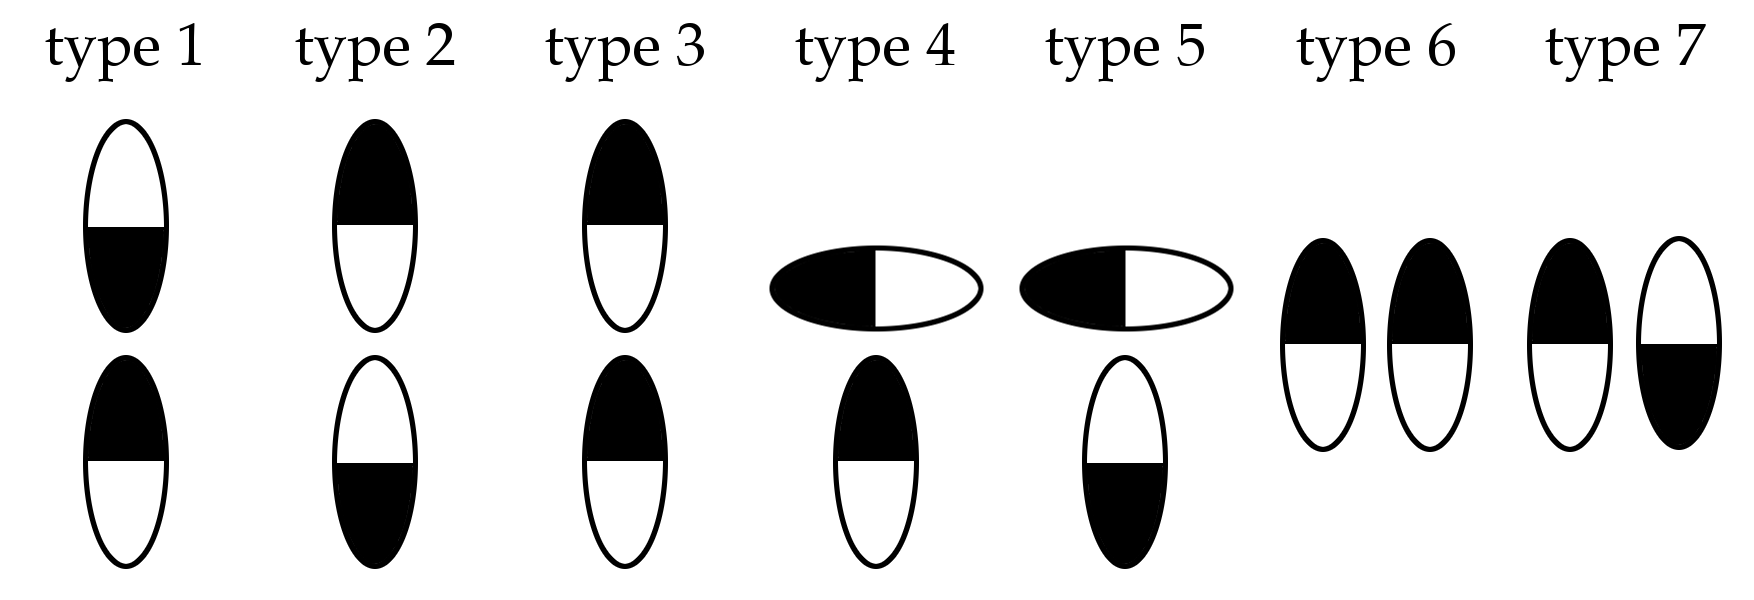
\includegraphics[width=\textwidth]{figures/introduction/classification}
	\nicecaption{Different two-molecule interaction types}{The black part refers to the FERM domain, the white to the kinase.}
	\label{methods:inttypes}
\end{figure}
%
%
%
\chapter{Setup}
\section{Protein structure}
All simulations have been done with starting configurations adapted from previous work in the group (C36 forcefield: \textcite{pap003}, Martini forcefield: \textcite{sara}). These configurations contain only a FERM-kinase fragment without the FAT domain and its linker (residues 35 to 686, PDB 2J0J \autocite{structFAK}).\\
As explained in \autoref{subsub:coarsegraining} the secondary structure of proteins have to be stabilized in Martini using elastic networks. This was set up by \textcite{sara}. It acts only between residues of the same domain with a force constant of 830 $\si{\kilo\joule\mole^{-1}\nano\meter^{-2}}$. Therefore the interface between FERM domain and kinase is not affected and the linker is still flexible.
\section{Setup 1 - FAK in solution}
\label{setup:setup1}
This setup contains a single FAK molecule in Martini structure, which was placed in a waterbox with ions to eliminate net charges. After a short equilibration the system was simulated for $20\,\si{\micro\second}$ at a temperature of $300\si{\kelvin}$. The standard parameters of the Martini forcefield were used as simulation parameters.
\section{Setup 2 - Free energy of basic patch}
\label{setup:setup2}
For this setup only a part of F2 (residues 107 to 219, referred as F2 lobe in the following), which contains the basic patch, was used. The lobe was placed above a single \pip{} embedded into a phosphatidylethanolamine (\pope{}) membrane (see \autoref{tobeadded}). After a short equilibration the F2 lobe was pulled slowly away from the membrane using a distance pull between the COM of the F2 lobe and the COM of \pip{}. This simulation was used to retrieve starting conformations for the umbrella windows.\\
The starting configuration was set up in C36 and transferred to a Martini (with PW) structure with provided transformation tools \autocite{backwardpy, PW}. In the Martini structures the mentioned elastic network was applied.\\
The number of umbrella windows was chosen accordingly to the sampling (between 90 and 120 windows). Each window was shortly equilibrated and then simulated for $6\,\si{\nano\second}$ in C36 and $10\,\si{\nano\second}$ in Martini (with PW). From the trajectories of the umbrella windows the free energy profile was calculated using \gromacs{} WHAM implementation \autocite{gromacsWHAMpaper}. For each forcefield five different profiles were obtained to estimate the statistical error.\\
The presented results are based on a total simulation time of $6.33\,\si{\micro\second}$ for Martini, $5.64\,\si{\micro\second}$ for Martini with PW and $3.88\,\si{\micro\second}$ for C36. The temperature in the simulation was $300\si{\kelvin}$. % C36: 1=180, 4.2=135, 5=102, 5.2=102, 6=127, Mart: 1=134, 2=126, 3=130, 4=113, 5=130, MartPol: alle=113
\section{Setup 3 - FAK on a \pip{} membrane}
\label{setup:setup3}
Setup 3 was adopted from \textcite{sara} and contains a single FAK molecule in Martini structure, which was placed on a phosphatidylcholine (\popc{}) and \pip{} (15\%) membrane. Ions were added to eliminate net charges. In contrast to \textcite{sara} the stabilizing force explained in \autoref{motivation} was applied to the protein.\\
Five different copies were simulated for $10\,\si{\micro\second}$ each with a temperature of $300\si{\kelvin}$.
\section{Setup 4 - FAK cluster}
In order to set up a cluster of multiple FAK molecules 25 different frames were chosen from setup 3 equidistant in time. The frames were arranged on a {5x5} grid. The stabilizing force was applied on each FAK molecule independently. After a short equilibration the system was simulated for $9\,\si{\micro\second}$. Five different copies (regarding to the arrangement of the frames) were set up, resulting in a total simulation time of $45\,\si{\micro\second}$. The temperature was set to $300\si{\kelvin}$.
\chapter{Results}
\label{results:umbrella}
In order to understand the falling of FAK onto the membrane the free energy profile of the binding of the basic patch to \pip{} was investigated. Since this binding is the main contact between FAK and the membrane in our model, a short report on the results is given at this point.\\
The profiles are obtained from setup 2. The reaction coordinate is the z component of the COM distance between \pip{} and the protein fragment. For each forcefield, C36, \martini{} and \martini{} with PW, the average profile out of the five copies together with the standard deviation can be found in \autoref{umbrella:profiles}. The range $6\,\si{\nano\metre} \le z \le 7\,\si{\nano\metre}$ was set as zero point.\\
%
%
%
\begin{figure}[hb]
	\centering
	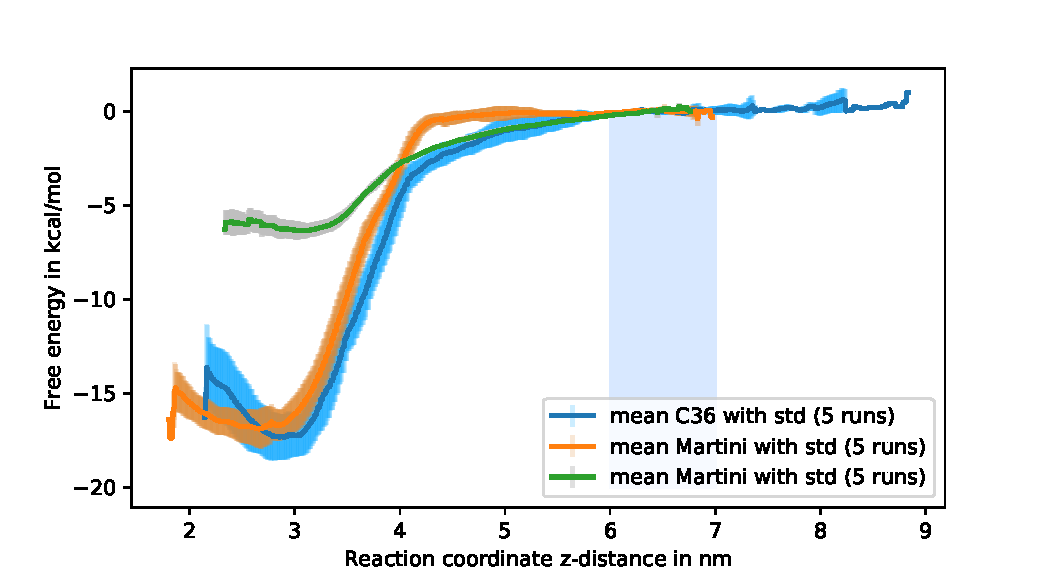
\includegraphics[width=.8\textwidth]{figures/results/umbrella}
	\nicecaption{Free energy profile of basic patch}{For each forcefield the average and standard deviation of the five copies is presented.}
	\label{umbrella:profiles}
\end{figure}
%
%
%
\\
Both, C36 and \martini{}, show a similar energy depth of $\approx 17 \si{\kilo Cal/\mole}$ and a similar slope between $3\,\si{\nano\metre} \le z \le 4\,\si{\nano\metre}$ . Certainly, \martini{} shows systematically more shallow wells than the all atom simulation. This can be attributed to the proposed underestimation of electrostatic forces due to the unpolar water beads (see \autoref{subsub:coarsegraining}). The difference at $z = 4.2\,\si{\nano\metre}$ originates from the different treatment of long range electrostatics: \martini{} uses a cut-off radius, C36 uses PME.\\ %TODO: maybe force switch function in martini? what about the kink in C36?
Also \martini{} with PW uses PME for long range electrostatic interactions and indeed it fits much better to the C36 profile for larger distances. However, the binding strength is crucially underestimated in Martini with PW.\\
The extent to which \martini{} reproduces the results from all-atom simulations is remarkable, even though the parameters for \martini{} were obtained from free energy calculations (see \autoref{subsub:coarsegraining})\\
\\
In the used starting configurations, the proteins are already bound to \pip{}. Therefore a correct binding strength and the shape near the minimum is of larger interest than a correct sampling of farther distances. In addition \martini{} with PW required a much higher computational effort. That is why we consider only the standard water model in the following simulations.

\subsection{Impacts of the stabilizing force}
In setup 3 a and setup 4 each protein was stabilized with an external force acting on the FERM domain (see \autoref{motivation}). Therefore the dependency of the used observables is examined below.\\
\\
The force has a mean value of $1.47\,\forceunit$ and a standard deviation of $13.13\,\forceunit$. It is skewed to positive values. This is expected since positive values of the force require negative elongations $\Delta z$. If the connecting vector of F1 and F2 $\vec{d}_F$ is parallel to the z-axis, larger negative deviations require a stretching of $d_F$, which suppress these forces. \\
\\
Linear regressions show that none of the quantities $d_F$, $d_\text{F1-N}$, $d_\text{F2-C}$ and CA have a remarkable correlation to the applied force. Here remarkable means that either the regression result was not significant or that the obtained slope was so small, that a change of two standard deviations in force would not change the quantity noticeably.\\
\\
Also the distances between residue pairs are tested for correlation with the applied force. To this end, 10 different proteins without neighbours were picked out of the trajectories of setup 4, each for $1\,\si{\micro\second}$. On this dataset a linear regression was performed for each residue pair. \autoref{force:contactmap} shows the calculated Pearson correlation coefficient (only significant correlations with Pearson $\left|r\right| > 0.3$). The mean value of the slope for the positive correlated pair distances is $20.3\,\si{\pico\newton/\nano\metre}$ and $-19.7\,\si{\pico\newton/\nano\metre}$ for the negative correlated pair distances. Thus, the force can have large influences on these pairs. However, not all observed contacts at the interface (compare to \autoref{free:contact}) are effected.
%
%
%
\begin{figure}
	\centering
	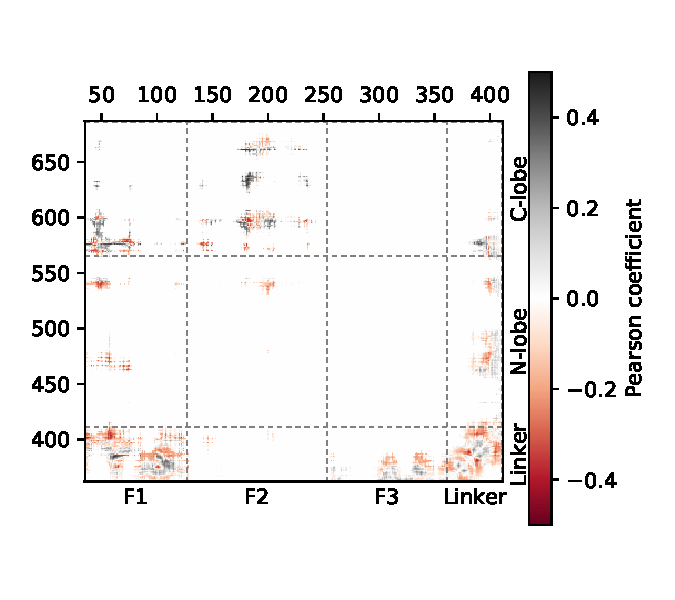
\includegraphics[width=.7\textwidth]{figures/results/interface_corr}
	\nicecaption{Correlations in contact map}{The contact map shows residue pairs, whose distance correlates with the applied force. The obtained slope is about $20\,\si{\pico\newton/\nano\metre}$.}
	\label{force:contactmap}
\end{figure}
%
%
%
\\
It is important to note that in this section only the observed quantities were tested for correlation with the force. It is however possible and probable, that due to this restriction, configurations or states are completely missing while others are over expressed. This effect can not be estimated, but should be kept in mind.
\end{document}